\begin{frame}[t]{ohmscher Widerstand}

    \textbf{Ziel - Darstellung von Bauteilkennlinie}
    
    \begin{spacing}{0.6} \begin{tiny}
    
    Das ohmsche Gesetz $U=R I$ lässt sich mit Hilfe eines kleinen Schaltungsexperimentes gut visualisieren und nachvollziehen. 
    Hierzu werden wir die folgende Schaltung aufbauen und den Stromverlauf über dem Widerstand darstellen. 
    \end{tiny} \end{spacing}
    \begin{spacing}{0.9} \begin{tiny}
    \begin{table}[h!]
      \begin{tabular}{p{3cm} p{7cm}}
        \hline
        \textbf{Erstellung des Schaltplans} & \\
        \hline \\
        \begin{minipage}{.3\textwidth}
          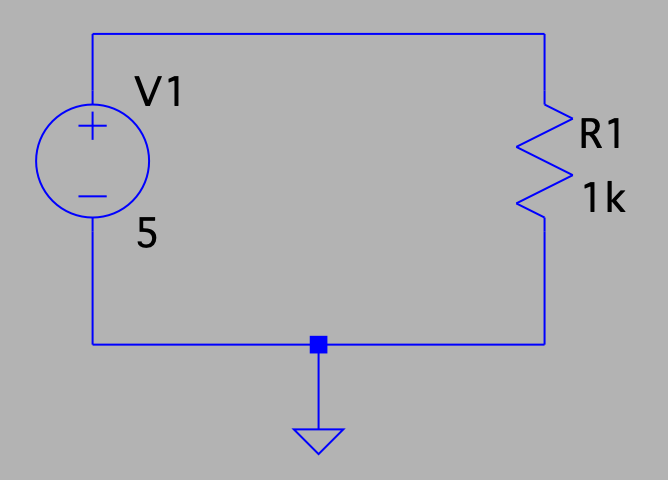
\includegraphics[width=\linewidth]{pictures/res.png}
        \end{minipage} 
        & 
        \begin{minipage}{.7\textwidth}
        \begin{itemize}
          \item Erstellt ein neues schematic (File $->$ new schematic)
          \item Speichert es direkt als neue Dateil ab (File $->$ save as)
          \item Öffnet den Bauteileditor (\textbf{F2}) und für eine Spannungsquelle hinzu (voltage)
          \item Öffnet erneut den Bauteileditor und für einen Widerstand hinzu (resistor bzw. EuropeanResistor fuer die bekannte Box-Darstellung)
          \item Fügt einen Masseknoten als Bezugsknoten hinzu (\textbf{F4}).
          \item Verdrahtet die Schaltung (\textbf{F3})
        \end{itemize}
        \end{minipage} 
        \\
         & \\
         \hline
         \textbf{Konfiguration der Simulation} & \\
         \hline \\
         \begin{minipage}{.3\textwidth}
          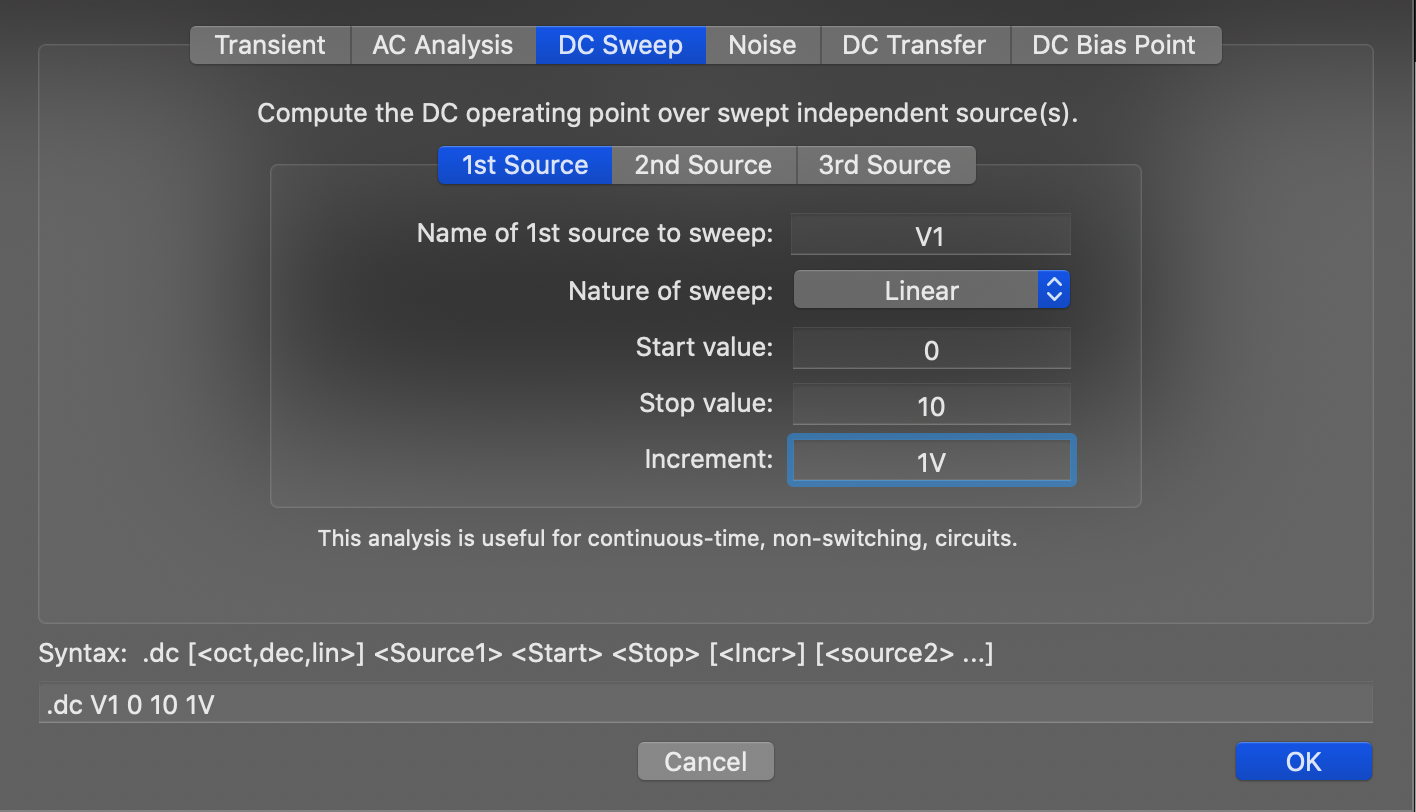
\includegraphics[width=\linewidth]{pictures/simulationcmd_1.png}
        \end{minipage} 
        & 
        \begin{minipage}{.7\textwidth}
        \begin{itemize}
          \item Im Menu Simulation, wählt \textbf{Edit simulation command} und wählt den DC Sweep. 
          \item Unser Ziel ist es den Stromverlauf über dem Widerstand zu simulieren
          \item Daher konfigurieren wir die Spannungsquelle \textbf{V1} mit einem \textbf{linearen} Sweep von 0 bis 10 V mit einer \textbf{Schrittweite} von 1V.
          \item Bestätigt mit \textit{OK} und fügt die Sumlationsansweisung dem schematic hinzu
        \end{itemize}
        \end{minipage} 
        \\
         & \\
         \hline
      \end{tabular}
    
    \end{table}
    
    \end{tiny} \end{spacing}
    
     \end{frame}
    
     \begin{frame}[t]{ohmscher Widerstand}
    
      \begin{spacing}{0.9} \begin{tiny}
      \begin{table}[h!]
        \begin{tabular}{p{5cm} p{5cm}}
          \hline
          \textbf{Simulation und Analyse} & \\
          \hline \\
          \begin{minipage}{.5\textwidth}
            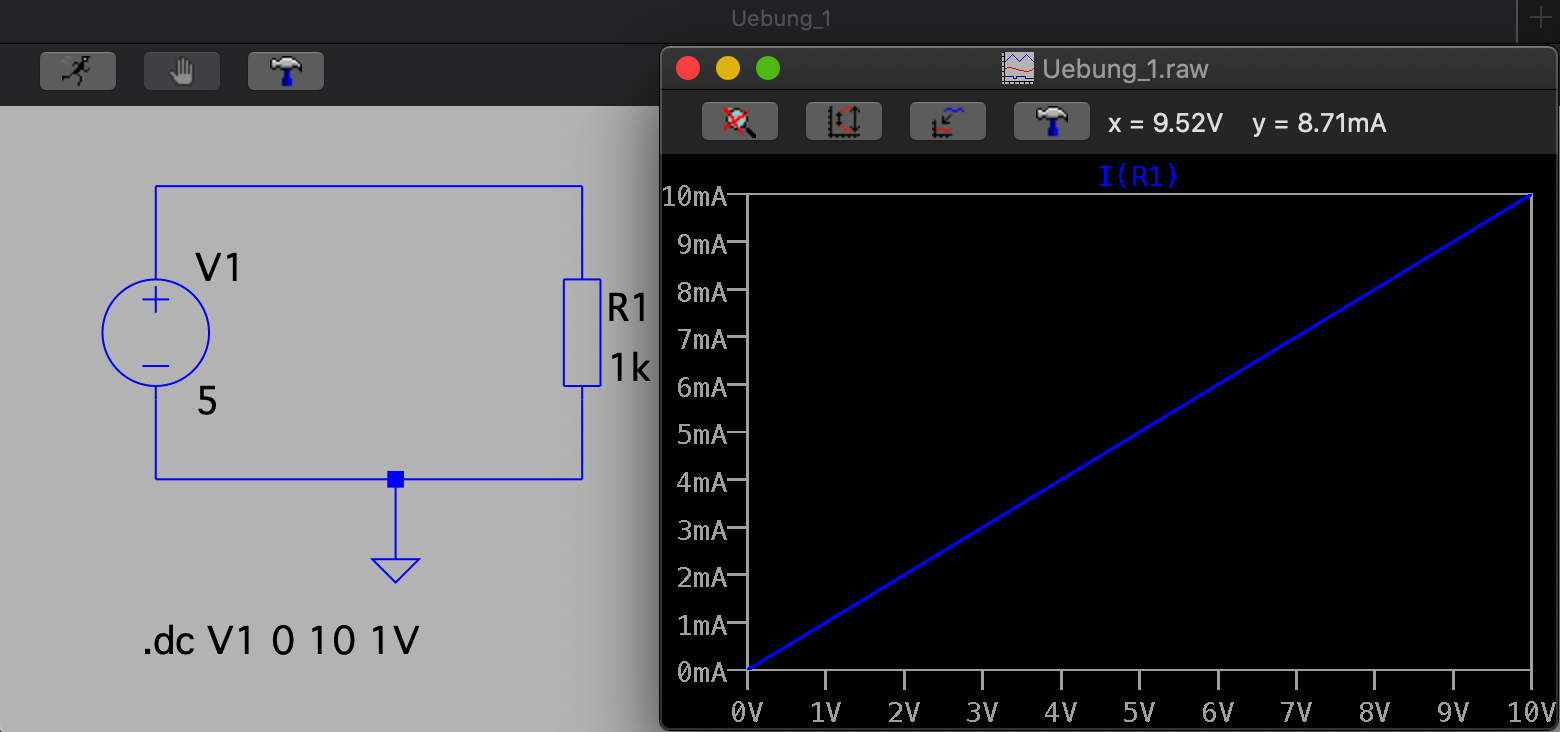
\includegraphics[width=\linewidth]{pictures/analysis.png}
          \end{minipage} 
          & 
          \begin{minipage}{.5\textwidth}
          \begin{itemize}
            \item Klickt auf 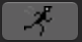
\includegraphics[scale=0.3]{pictures/run.png} (run) und LTspice startet die Simulation
            \item Der waveform viewer öffnet sich - ihr könnt auf zwei Arten Strom, Spannung und Leistungen aus eurer Schaltung anzeigen lassen. \newline\newline
            \textbf{Im schematic} könnt ihr über ein Bauteil mit der Maus fahren und es erscheint eine Stromzange\newline\newline
            \textbf{Im schematic} könnt ihr über ein Bauteil mit der Maus fahren, Shift gedrückt halten und es erscheint eine Leistungsmessanzeige\newline\newline
            \textbf{Im schematic} könnt ihr über eine Knoten mit der Maus fahren und es erscheint ein Spannungsmesser\newline\newline
            \textbf{Im waveform viewer} könnt ihr über rechten Mausklick $->$ add trace die verfügbaren Messtellen direkt auswählen
            \item Wir wählen \textbf{I(R1)}, den Strom durch unseren Widerstand R1. 
          \end{itemize}
          \end{minipage} 
          \\
        \end{tabular}
      \end{table}
    \end{tiny} \end{spacing}
    
      \begin{spacing}{0.9} \begin{tiny}
        \begin{table}[h!]
          \begin{tabular}{p{10cm} }
            \hline
            \textbf{Ergebnis und Auswertung} \\
            \hline \\    
            Wie zu erwarten liefert dieses einfache Beispiel den Zusammenhang zwischen Strom, Spannung und Widerstand. Probiert an dieser Stelle gerne die Spannung, Schrittweite
            zu variieren oder weitere Werte im waveform viewer anzueigen zu lassen.
          \end{tabular}
        \end{table}
      \end{tiny} \end{spacing}
      
       \end{frame}